%%%%%%%%%%%%%%%%%%%%%%%%%%%%%%%%%%%%%%%%%
% Beamer Presentation
% LaTeX Template
% Version 2.0 (10/06/16)
%
\documentclass[aspectratio=169]{beamer}
\beamertemplatenavigationsymbolsempty%
\usepackage{textpos}
\usefonttheme[onlymath]{serif}
\usepackage{amsmath}
\usepackage{empheq}
\usepackage{fontspec}
\usepackage{hyperref}
\usepackage{textcomp}
\usepackage{multirow}
\usepackage[document]{ragged2e}
\setsansfont{Linux Biolinum O}
%\setmainfont{Gentium}
\usetheme{Rochester}% theme
\usecolortheme{seahorse}
\colorlet{beamer@blendedblue}{green!40!black}
%\setbeamertemplate{navigation symbols}{}
%\setbeamertemplate{footline}[frame number]
\setbeamertemplate{footline}{% hide total number of slides
  \hfill% 
  \usebeamercolor[fg]{page number in head/foot}% 
  \usebeamerfont{page number in head/foot}% 
  %\insertframenumber%
  \insertpagenumber
  \kern1em\vskip2pt% 
}
\setbeamertemplate{itemize items}[circle]
\hypersetup{
    colorlinks = true,
    urlcolor = cyan
}

% Define color "lightgreen" for highlighting equarions
\definecolor{lightgreen}{HTML}{90EE90}

\addtobeamertemplate{frametitle}{}{%
\begin{textblock*}{100mm}(.93\textwidth,-0.77cm)

\includegraphics[height=0.77cm]{figures/csu-logo.png}
\end{textblock*}
\begin{textblock*}{100mm}(.995\textwidth,-1.6cm)

\includegraphics[height=0.8cm]{figures/Lang_candidate_for_NOvA-logo-2.eps}
\end{textblock*}}

\title{Iterative Unfolding Optimization with the Mean Squared Error Metric}
\date[today]{Finding-numu Meeting\\ \today}
\author{Shih-Kai Lin}
\institute{Colorado State University}
\usepackage{multicol} % 
%\usepackage{animate}  % animation
\usepackage{amsmath,amsfonts,amssymb} % This makes the equations appears better 

\titlegraphic{
\includegraphics[height=1cm]{figures/Lang_candidate_for_NOvA-logo-2.eps}\hspace*{6cm}~%
   
\includegraphics[height=1cm]{figures/csu-logo.png}
}

\begin{document}
%The title
\begin{frame}
\titlepage
\end{frame}

\begin{frame}{Recap}
  \begin{itemize}
    \item The standard metric in the ND group used by all analyses requiring unfolding is the average global correlation coefficient\footnote[frame]{Stefan Schmitt, ``Data Unfolding Methods in High Energy Physics''},
      \begin{equation} \label{eq:1}
        \rho_{avg}=\frac{1}{M}\sum_{j=1}^{M}\sqrt{1-\frac{1}{\pmb{V}_{jj}(\pmb{V}^{-1})_{jj}}}
      \end{equation}
    , where $M$ is the number of bins and $\pmb{V}$ is the covariance matrix in true space inferred by the unfolding algorithm.
    \item For analyses with tens of bins, this is a convenient metric. However, for an analysis with thousands of bins, this metric turned out to be infeasible.
  \end{itemize}
\end{frame}

\begin{frame}{Infeasibility of Average Global Correlation Coefficient for Many-Bin Analyses}
  \begin{columns}
    \begin{column}{.65\textwidth}
    Inverting a covariance matrix this large turns out to be very tricky.
    \begin{itemize}
      \item The covariance matrices all have astronomical \textcolor{red}{condition numbers} (i.e., ill-conditioned or nearly singular).
      \item Numerical inversion is still possible but subject to an arbitrary, small cut-off number, or tolerance, brought into play by SVD.
      \item Forcefully getting the calculation through results in numerical instability, such as negative values in square root in Eq.~\ref{eq:1}. Removing unphysical values, results are shown to the right. No clear minimum is observed.
    \end{itemize}
    \end{column}
    \begin{column}{.35\textwidth}
      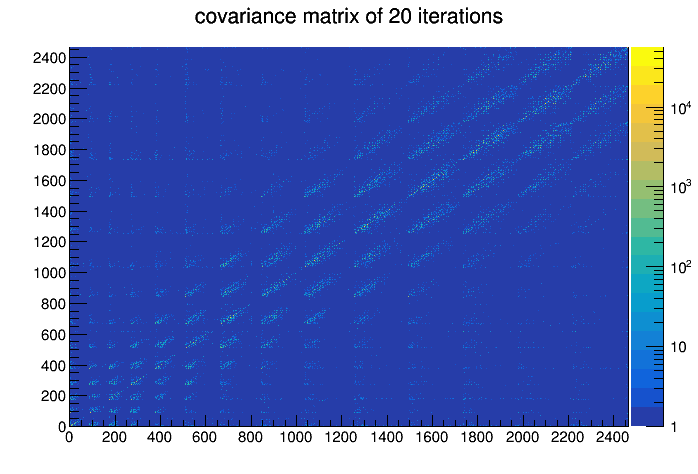
\includegraphics[width=\textwidth]{figures/cov_mat_iter20.png} \\
      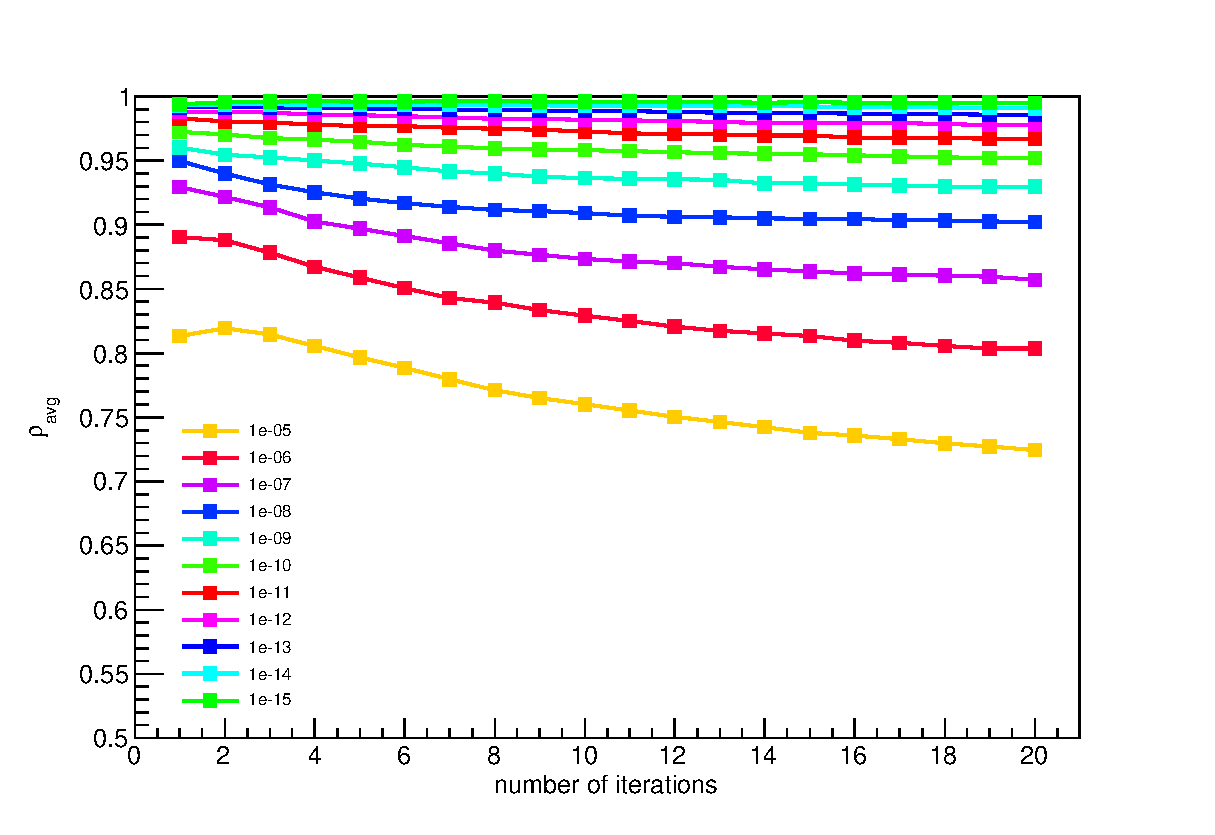
\includegraphics[width=\textwidth]{figures/avg_rho.eps}
    \end{column}
  \end{columns}
\end{frame}

\begin{frame}{Reference}
  \begin{columns}
    \begin{column}{.5\textwidth}
      Most of the contents in this document are taken from this textbook, especially Chapter 11 dedicated to unfolding.
    \end{column}
    \begin{column}{.5\textwidth}
      \centering
      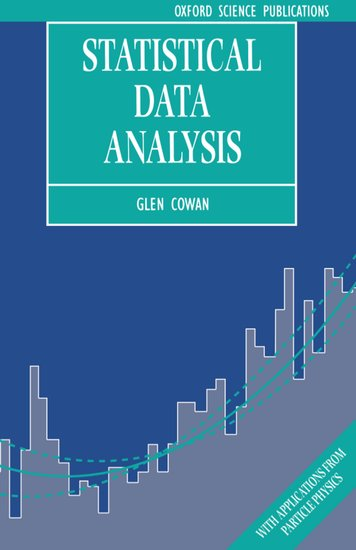
\includegraphics[height=\textheight]{figures/cowan_front_cover.jpeg}
    \end{column}
  \end{columns}
\end{frame}

%\begin{frame}{Mean Squared Error \& \\Bias-Variance Decomposition}
%Suppose $\theta$ is the a true parameter to be estimated, and $\hat{\theta}$ is an estimator of the parameter.
%The mean squared error (MSE) can be decomposed into a sum of variance and bias squared.
%\begin{eqnarray}
%MSE &=& E[(\hat{\theta}-\theta)^2]\nonumber\\
%&=& E[\hat{\theta}^2-2\hat{\theta}\theta+\theta^2] = E[\hat{\theta}^2] -2\theta E[\hat{\theta}]+\theta^2 \nonumber\\
%&=& (E[\hat{\theta}^2]-E[\hat{\theta}]^2)+(E[\hat{\theta}]^2-2\theta E[\hat{\theta}]+\theta^2) \nonumber\\
%&=& V[\hat{\theta}]+b^2
%\end{eqnarray}
%, where $b=E[\hat{\theta}]-\theta$ is the bias of the estimator.
%\vfill
%This is a very common metric in machine learning as well.
%\end{frame}
%
%\begin{frame}{Mean Squared Error in the Context of Unfolding}
%Given a true histogram $\pmb{\mu}=(\mu_1,...,\mu_M)$, where $\mu_i$'s are true counts in the $i$-th bin, $i=1,...,M$, unfolding can be viewed as a procedure that outputs a vector of estimators for the bin counts $\pmb{\hat{\mu}}=(\hat{\mu}_1,...,\hat{\mu}_M)$.
%
%Denoting the mean squared error for the $i$-th bin $MSE_i$, MSE for the histogram can be defined as
%\begin{eqnarray}
%  MSE &=& \frac{1}{M}\sum_{i=1}^M MSE_i \nonumber\\
%  &=& \frac{1}{M}\sum_{i=1}^M U_{ii}+\hat{b}_i^2
%\end{eqnarray}
%, where $U_{ii}=cov[\hat{\mu}_i,\hat{\mu}_i]$ and $\hat{b}_i$ is an estimator of $E[\hat{\mu}_i]-\mu_i$.
%\end{frame}
%
%%=================================================================
%\begin{frame}{Mean Squared Error in the Context of Unfolding (Cont.)}
%Very often one wants to estimate more accurately bins with smaller statistical uncertainties. In this case, weighted MSE can be used:
%\begin{eqnarray}
%  weighted \quad MSE &=& \frac{1}{M}\sum_{i=1}^M \frac{MSE_i}{\hat{\mu}_i} \nonumber\\
%  &=& \frac{1}{M}\sum_{i=1}^M \frac{U_{ii}+\hat{b}_i^2}{\hat{\mu}_i}
%\end{eqnarray}
%\end{frame}
%
%
%%=================================================================
%\begin{frame}{Practical Considerations with \texttt{RooUnfold}}
%  \texttt{RooUnfold} calculates the full covariance matrix $U_{ij}$. However, as far as I know, it does not calculate bias $\hat{b}_i$.
%  
%  Three options in my mind.
%  \begin{enumerate}
%    \item Handwave the expectation value calculation by assuming that the statistical uncertainties are negligible, i.e., $b_i=E[\hat{\mu}_i]-\mu_i \approx \hat{\mu}_i-\mu_i \approx \hat{b}_i$.
%  \end{enumerate}
%  If we really want to beat the problem to death, we can:
%  \begin{enumerate}
%    \setcounter{enumi}{1}
%    \item Generate toy MC spectra by varying counts in each bin of the true spectrum by Poisson (not reco, since reco undergoes smearing), smear them with the response matrix, do unfolding one by one, and calculate the bias.\\ \textcolor{red}{This is computationally infeasible.}
%    \item Calculate the bias faithfully. See the next slides.
%  \end{enumerate}
%\end{frame}
%
%
%%=================================================================
%\begin{frame}{Covariance Matrix Calculation in \texttt{RooUnfoldBayes}}
%From Tim's document, \href{https://arxiv.org/pdf/1105.1160.pdf}{Unfolding algorithms and tests using RooUnfold}, Eq's (2), (3), and (4) (sorry, now Tim's notation!):\\
%\footnotesize
%\textcolor{blue}{unfolding matrix:}
%\begin{equation}
%\hat{n}(C_i)=\sum_{j=1}^{n_E}M_{ij}n(E_j)\text{ where }M_{ij}=\frac{P(E_j|C_i)n_0(C_i)}{\epsilon_i\sum_{l=1}^{n_C}P(E_j|C_l)n_0(C_l)}
%\end{equation}
%\textcolor{blue}{error propagation matrix:}
%\begin{equation}\label{err_mat}
%\frac{\partial \hat{n}(C_i)}{\partial n(E_j)}=M_{ij}+\sum_{k=1}^{n_E}M_{ik}n(E_k)\left( \frac{1}{n_0(C_i)}\frac{\partial n_0(C_i)}{\partial n(E_j)}-\sum_{l=1}^{n_C}\frac{\epsilon_l}{n_0(C_l)}\frac{\partial n_0(C_l)}{\partial n(E_j)}M_{lk} \right)
%\end{equation}
%\textcolor{blue}{covariance matrix on the unfolded distribution:}
%\begin{equation}
%V(\hat{n}(C_k),\hat{n}(C_l))=\sum_{i,j=1}^{n_E}\frac{\partial \hat{n}(C_k)}{\partial n(E_i)}V(n(E_i),n(E_j))\frac{\partial \hat{n}(C_l)}{\partial n(E_j)}
%\end{equation}
%
%\end{frame}
%
%
%%=================================================================
%\begin{frame}{Bias Calculation with Iterative Unfolding}
%Back to Cowan's \href{http://www.ippp.dur.ac.uk/Workshops/02/statistics/proceedings/cowan.ps}{document} and notation, a generic formula for bias is
%\begin{equation}
%\hat{b}_i=\sum_{j=1}^{N}\frac{\partial \hat{\mu}_i}{\partial n_j}\left(\sum_{l=1}^M R_{jl}\hat{\mu}_l-n_j\right)
%\end{equation}
%, where $\frac{\partial \hat{\mu}_i}{\partial n_j}$ is the error propagation matrix given by Eq.~(\ref{err_mat}), $R$ is the response matrix, $\pmb{\hat{\mu}}$ is the unfolded spectrum, and $\pmb{n}$ is the measured reco spectrum.
%\end{frame}
%
%
%%=================================================================
%\begin{frame}{Going Forward with This Metric}
%Given Connor's variance and bias studies, if we go with this metric, we can expect some minimum before 5 iterations.\\
%If we can explain away with option 1, we will close this task in no time.
%\end{frame}


\end{document}